\documentclass[12pt,a4paper,faculty=ea,language=en]{ugent-doc}

\usepackage{todonotes}

\usepackage{xurl}
\usepackage[expansion=false]{microtype}

\usepackage{hyperref}
\hypersetup{
    colorlinks=true,
    breaklinks=true,
    urlcolor=black,
    linkcolor=black,
    citecolor=black
}

\usepackage{graphicx}
\graphicspath{{figures/}}

\usepackage{float}
\usepackage{pgfgantt}

\usepackage{listings}
\usepackage{xcolor}
\usepackage{fancyvrb}

\lstset{
    language=C,
    basicstyle=\ttfamily\small,
    keywordstyle=\color{blue},
    stringstyle=\color{red},
    commentstyle=\color{green!70!black},
    numbers=none,
    numberstyle=\tiny\color{gray},
    stepnumber=1,
    numbersep=10pt,
    showspaces=false,
    showstringspaces=false,
    showtabs=false,
    tabsize=2,
    captionpos=b,
    breaklines=true,
    breakatwhitespace=false,
}

\usepackage{amsmath}

\usepackage{amsthm}

\usepackage{amssymb}
\usepackage{booktabs}


\setlength{\parindent}{0pt}
\setlength{\parskip}{0.6em}

\hyphenation{cor-rect-heid}

\thetitle{\color{ugentblue}Efficient Design Space Exploration for Sustainable Processor Architectures}

\infoboxa{\bfseries\large Research internship}

\infoboxb{Promotor:
\begin{tabular}[t]{l}
    Prof.\ dr.\ ir.\ Lieven Eeckhout\\
\end{tabular}
\\[0.5em]
Assistant:
\begin{tabular}[t]{l}
    ir.\ Ruben Verheyden\\
\end{tabular}
}

\infoboxc{Student:
\begin{tabular}[t]{lll}
    Jaco Lagrange & \href{mailto:jaco.lagrange@ugent.be}{jaco.lagrange@ugent.be}\\
\end{tabular}
}

\infoboxd{Academic year: 2026--2027}

\begin{document}
\maketitle

{\hypersetup{hidelinks}\tableofcontents}
\newpage
\section{Background}
This internship works further on the research done in the paper \emph{ASI: A Unifying Metric to Assess and Improve Processor Microarchitecture Sustainability}~\cite{asi2026}. This section summarizes the ASI metric itself, why it is naturally paired with a speedup Pareto front, the Sniper simulator used to evaluate candidate designs, and why exploring the resulting design space requires more than a single search algorithm.

\subsection{Sustainable Processor Microarchitectures}
Information and communication technology is responsible for a significant and growing share of global carbon emissions, and processor microarchitecture design plays a direct role in that footprint: every design decision -- cache sizes, reorder buffer depth, branch predictor complexity, and so on -- trades off performance against the chip area and power that ultimately determine a design's \emph{embodied} footprint (manufacturing) and \emph{operational} footprint (use-phase energy). A subtlety that makes this optimization hard is the \emph{rebound effect} (Jevons' paradox): a more efficient design is often used more intensively, so a design that looks greener when compared at a fixed amount of work can end up doing more overall harm once its higher efficiency causes it to be used more.\cite{asi2026} Assessing sustainability therefore requires reasoning about both a fixed-work and a fixed-time usage scenario at once, not just picking the design with the lowest energy or power in isolation.

\subsection{The Architectural Sustainability Indicator (ASI)\cite{asi2026}}
ASI builds on FOCAL~\cite{focal2024}, which compares a candidate design $X$ against a reference design $Y$ using a \emph{Normalized Carbon Footprint} (NCF): a weighted sum of $X$'s chip area relative to $Y$ (a proxy for embodied footprint) and $X$'s energy or power relative to $Y$ (a proxy for operational footprint). Energy is used for the footprint under a fixed-work scenario (both designs do the same amount of work), while power is used for the footprint under a fixed-time scenario (both designs run for the same amount of time, so a faster design also does more work) -- this is exactly what lets FOCAL, and by extension ASI, expose the rebound effect instead of hiding it. A weighting factor $\alpha \in [0,1]$ sets how much the embodied footprint counts relative to the operational one (e.g. $\alpha \approx 0.8$ for mobile/embedded devices where manufacturing dominates, $\alpha \approx 0.2$ for always-on devices where energy use dominates).

Rather than reporting these two NCF values separately, ASI folds them into a single higher-is-better number relative to the reference design ($\mathrm{ASI} = 1$):
\begin{equation}
    \mathrm{ASI} = \frac{1 - \alpha A_n}{(1-\alpha) P_n},
\end{equation}
where $A_n$ and $P_n$ are the candidate design's chip area and power, each normalized to the reference design's. Whether a design counts as sustainable then depends on how ASI compares to $1$ \emph{and} to the normalized execution time $T_n$ (equivalently, the inverse of the speedup $S = 1/T_n$), as summarized in Table~\ref{tab:asi-regions}.

\begin{table}[H]
    \centering
    \begin{tabular}{ll}
        \toprule
        Strongly sustainable & $\mathrm{ASI} > \max(1, T_n)$ \\
        Unsustainable & $\mathrm{ASI} < \min(1, T_n)$ \\
        Weakly sustainable & $\min(1, T_n) < \mathrm{ASI} < \max(1, T_n)$ \\
        \bottomrule
    \end{tabular}
    \caption{Classifying a design's sustainability from its ASI value and normalized execution time $T_n$~\cite{asi2026}.}
    \label{tab:asi-regions}
\end{table}

A strongly sustainable design reduces the footprint under both scenarios; a weakly sustainable one only reduces it under one of the two (i.e. it is prone to the rebound effect); an unsustainable one increases the footprint under both. Because $T_n$ (equivalently speedup) appears directly in these thresholds, ASI cannot be read in isolation -- it is only meaningful together with the performance change it comes with. Classifying a design this way needs both ASI and speedup at once, so plotting ASI against speedup is the natural way to visualize a design's sustainability profile: it turns the three qualitative categories above into geometric regions of a single 2D plane, with the reference design sitting at $(1,1)$. This is also why design space exploration in this project targets the \emph{Pareto front} of ASI versus speedup rather than optimizing either metric alone: a point is Pareto-optimal if no other explored configuration is simultaneously at least as good on both axes. Sweeping out that front, instead of collapsing sustainability and performance into one scalar objective, is what lets a designer see the full range of available trade-offs -- from "almost free" sustainability gains that cost negligible performance, to designs that push ASI much higher at a real performance cost -- and pick the one that fits their constraints, rather than committing up front to a fixed trade-off weighting. It is also what directly exposes the rebound effect: a design that looks attractive on energy alone can still turn out to be only weakly sustainable or outright unsustainable once its speedup is accounted for, which a single-objective search would not reveal.

\subsection{The Sniper Simulator}
Evaluating a candidate microarchitecture's speedup, and its area/power proxies for $A_n$ and $P_n$, requires actually simulating it. This project uses Sniper~\cite{sniper2014}, a fast, validated multicore x86 simulator developed at Ghent University that combines interval-based and cycle-level core models to estimate performance, and McPAT~\cite{mcpat2009} to estimate the corresponding chip area and power at a given technology node. Each candidate design point is therefore a full Sniper configuration (cache hierarchy, reorder buffer/dispatch width, branch predictor, etc.), and evaluating it means running the benchmark suite through Sniper and McPAT to obtain the (speedup, ASI) pair used to place that point on the Pareto front.

\subsection{Design Space Exploration at Scale}
\label{sec:dse-scale}
The microarchitectural parameters exposed for exploration (cache sizes and associativities, branch predictor type and its type-specific knobs, reorder buffer window/dispatch/commit width, and so on) already combine into on the order of $10^8$ candidate configurations. Since every point on that surface requires an actual detailed Sniper run across the full benchmark suite, exhaustively simulating the space is infeasible, and even a single fixed search heuristic is unlikely to be the most sample-efficient choice across every region of it. The goal of this internship is to implement and compare several complementary search strategies for tracing the ASI-versus-speedup Pareto front, and to evaluate how much of the true front each recovers for a given simulation budget.

\newpage

\section{Quantifying Pareto Front Quality}
Section~\ref{sec:search-strategies} compares several search strategies for tracing the ASI-versus-speedup Pareto front under a fixed simulation budget, which raises the question of how to decide that one recovered front is better than another. Unlike a single-objective search, where two runs can simply be ranked by their best objective value, a Pareto front is a set of trade-off points rather than a single number, so "better" has to account for both how close the front gets to the true, unknown optimum (convergence) and how well it covers the range of available trade-offs (spread). This section introduces the quality indicators used throughout the rest of this work.

\subsection{Hypervolume}
\label{sec:hv}
The hypervolume (HV) indicator measures the area of the ASI-versus-speedup plane dominated by a Pareto front, i.e. the area between the front's staircase and a fixed reference point -- the bigger that area, the better the front, since it means the front reaches further out on both axes at once~\cite{zitzler1999,guerreiro2021}. This project uses the origin $(0,0)$ as reference point:
\[
HV(P) = \sum_{i} \max(0, \mathrm{asi}_i) \cdot \max\big(0, \mathrm{speedup}_i - \mathrm{speedup}_{i-1}\big),
\]
with the points of $P$ sorted by ascending speedup. Keeping the reference point fixed at the origin, rather than deriving it from each run's own worst point, means the same reference is used across every strategy and every run, making their hypervolumes directly comparable, and it lets a point with negative ASI or speedup still stand on the front without contributing to HV on the axis where it falls below zero.

\subsection{Limitations of Hypervolume: Coverage and Clustering}
Hypervolume summarizes both the convergence and the spread of a front into a single number, but that same aggregation is also its weakness: two fronts with a comparable hypervolume can still differ substantially in how their points are distributed across the trade-off space. Because HV is dominated by the outermost points on the staircase, a front can score well while leaving large stretches of the ASI-versus-speedup plane completely uncovered, i.e. regions where no configuration on the front offers a trade-off at all. Figure~\ref{fig:hv-clustering} shows such a case:
\begin{figure}[H]
\centering
\includegraphics[width=0.48\textwidth]{~/school/stage-reports/images_results/ML24MiB_ML2_CCl_MIP_EI_hybrid_7init/mesmo_phase/pareto_final.png}
\caption{A recovered Pareto front with a competitive hypervolume that nonetheless leaves two clearly visible gaps in speedup where no point on the front provides a trade-off.}
\label{fig:hv-clustering}
\end{figure}
The points cluster into a small number of tight groups, separated by two regions with no points at all. Adding points inside those gaps would improve coverage of the design space, yet if they fall close to the existing staircase they add only marginally to the hypervolume, so HV alone gives little incentive to fill them. Consequently, hypervolume should not be used in isolation to judge a front's quality: it needs to be complemented by the number of points on the front and by a manual check of how many distinct regions of the trade-off space those points actually populate.

\section{Search strategies}
\label{sec:search-strategies}
This section explains and compares the different strategies used to explore the front.
\subsection{Evolutionary}
Evolutionary search algorithms mimic natural selection: a population of candidate solutions evolves over generations through selection, mutation and crossover, rather than climbing the objective surface (the landscape formed by the objectives being optimized -- here, ASI and speedup -- as a function of configuration) from a single starting point the way gradient- or hill-climbing-based methods do. This makes them more robust in non-convex search spaces, where hill climbing tends to get stuck in local optima, and it extends naturally to the multi-objective case by evolving an entire population of trade-off points at once instead of a single best solution, which is exactly what is needed to trace out a Pareto front.
The search strategy that was chosen is \emph{COLE: Compiler optimization level exploration}~\cite{cole2008}, an algorithm initially made for compiler space search. It is based on the SPEA2 algorithm \cite{spea2001}.
\subsubsection{COLE}
\label{cole}
COLE searches with several populations of entities in parallel rather than just one, where each entity is a candidate configuration, i.e. one specific setting of the microarchitectural parameters introduced in Section~\ref{sec:dse-scale} (cache sizes, branch predictor, reorder buffer width, etc.). Every generation, the Pareto-optimal entities of each population are kept in that population's archive; the next generation is then bred from the archive by binary-tournament selection, mutation and crossover, with a small migration probability letting entities move between populations so that one population's progress can seed another's. This repeats for a fixed number of generations, after which the per-population Pareto frontiers are merged into a single overall Pareto frontier, as shown in Figure~\ref{fig:cole-framework}.
\begin{figure}[H]
\centering
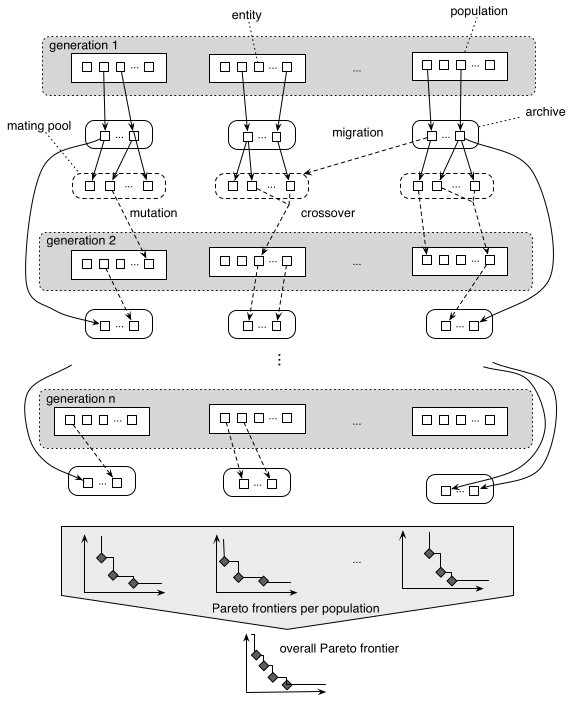
\includegraphics[width=0.8\textwidth]{cole_framework.png}
\caption{The COLE multi-objective optimization framework. Reproduced from Hoste and Eeckhout~\cite{cole2008}.}
\label{fig:cole-framework}
\end{figure}
It is important to note that each generation can be fully parallelized on its own, since all of its configurations can be run at the same time. This is done using the Titan cluster.
\subsubsection{Results}
\subsection{Bayesian Optimization}
Unlike evolutionary search, which requires evaluating a whole population of real configurations every generation, Bayesian optimization fits a cheap probabilistic surrogate model to the data already collected. Each new real evaluation is then used to refine that model and make better-informed guesses.
\subsubsection{MESMO: Max-value entropy search for multi-objective Bayesian optimization}
\label{mesmo}
MESMO~\cite{mesmo2019} is the algorithm used. It fits one Gaussian-process (GP) surrogate model per objective (ASI and speedup), trained on all configurations actually evaluated on Sniper so far; before any such data exists, an initial batch of configurations is run to give the models something to learn from. From there, the process repeats: the GPs are refitted on all real results gathered so far, a large pool of candidate configurations is proposed -- some being small variations on the configurations currently on the Pareto front, the rest fresh random guesses -- and every candidate is scored by an acquisition function that estimates how much a real evaluation at that candidate would help narrow down the true, unknown Pareto front. Only the candidates with the highest scores are then actually run on Sniper, and the resulting real measurements are added to the data used to refit the GPs in the next iteration.

The acquisition function estimates this expected benefit as follows. At any given configuration, the GP posterior does not give a single predicted value for ASI or speedup but a distribution of plausible values; the entropy of that distribution measures how uncertain the model still is there. The scoring procedure works with several imagined ``worlds'', each one a specific guess at what the true ASI and speedup values are for every configuration in the candidate pool, drawn at random from the GPs' current distributions (so a world consistent with everything measured so far, but not an actual measurement). For each imagined world, the Pareto front of that world's guessed values is computed over the whole candidate pool, exactly as it would be for real data; this gives one hypothetical Pareto front per world. Because that front is, by definition, the best set of trade-offs among the guessed values of \emph{all} candidates in that world, no single candidate's own guessed value in that world can be better than what the front already shows for it -- it is either on the front or dominated by it.

Now take one specific candidate configuration whose acquisition score is being computed, and one imagined world. Before looking at that world's front, the model's belief about this candidate's true value is the full, uncertain GP distribution. The front computation is then temporarily treated as if that one imagined world were the real one: under that assumption, any value for this candidate that would dominate the front is impossible, since the front already represents the best that world allows, so only values dominated by (or on) the front remain possible. Restricting the belief to only those possible values is the same operation as truncating a distribution once an upper limit on it becomes known, and it can be computed exactly. The resulting truncated distribution is less uncertain (lower entropy) than the original one, and the size of that drop in entropy is what this one world tells us about how informative it would be to actually evaluate the candidate. Since one imagined world is just one guess among many, this is repeated for several independently imagined worlds, and the entropy drops they each give for the candidate are averaged into that candidate's final score. Every candidate in the pool is scored this way, so the ones with the highest average expected information gain can be picked out and sent for real evaluation on Sniper.
\subsubsection{Results}
\subsection{Hybrid}
MESMO (Section~\ref{mesmo}) quickly reaches a reasonably good, though suboptimal, Pareto front, but its convergence slows sharply afterwards. COLE (Section~\ref{cole}), by contrast, starts from a randomly initialized population and only reaches a comparable front after many more generations. The hybrid strategy is designed to combine the strengths of both, rather than committing to either one for the whole simulation budget: MESMO is run first to reach a decent front quickly, and that front is then handed over to COLE to refine and expand further.

The first phase runs MESMO exactly as described in Section~\ref{mesmo}, except that instead of running for a fixed number of iterations, it is stopped as soon as the front's hypervolume (Section~\ref{sec:hv}) has stopped improving for a number of consecutive iterations. This early-stopping criterion targets precisely the later MESMO iterations that are responsible for its slow convergence, so the search moves on to the second phase once the model's guesses stop paying off rather than continuing to refine them at a diminishing rate.

The second phase runs COLE (Section~\ref{cole}), but instead of starting from an entirely random initial population, its populations are seeded with the front reached by MESMO in the first phase, together with any configurations retained by the parameter-screening pass described in Section~\ref{sec:preeval}, where that pass is used. Every configuration MESMO already evaluated is also carried over rather than re-evaluated, so the second phase continues exploring from where the first left off instead of repeating work already done. The remaining population slots not filled by these seed configurations are still initialized randomly, exactly as in the standalone COLE strategy, so the search space continues to be explored broadly rather than narrowing prematurely around MESMO's front.

Because both phases evaluate configurations on the same simulator and are judged by the same hypervolume metric, the two phases are reported as a single continuous search rather than two separate ones, with the point at which MESMO hands off to COLE marked explicitly, so the effect of the switch on convergence speed can be seen directly.
\subsubsection{Results}

\begin{thebibliography}{9}
\bibitem{asi2026}
    J. Roelandts, A. Naithani, and L. Eeckhout, "ASI: A Unifying Metric to Assess and Improve Processor Microarchitecture Sustainability," in Proc. 2026 IEEE Int. Symp. Performance Analysis of Systems and Software (ISPASS), Seoul, South Korea, 2026, pp. 495--506.
\bibitem{focal2024}
    L. Eeckhout, "FOCAL: A first-order carbon model to assess processor sustainability," in Proc. 29th ACM Int. Conf. on Architectural Support for Programming Languages and Operating Systems (ASPLOS), Volume 2, 2024, pp. 401--415.
\bibitem{sniper2014}
    T. E. Carlson, W. Heirman, S. Eyerman, I. Hur, and L. Eeckhout, "An evaluation of high-level mechanistic core models," ACM Trans. Archit. Code Optim., vol. 11, no. 3, Aug. 2014.
\bibitem{mcpat2009}
    S. Li, J. H. Ahn, R. D. Strong, J. B. Brockman, D. M. Tullsen, and N. P. Jouppi, "McPAT: an integrated power, area, and timing modeling framework for multicore and manycore architectures," in Proc. 42nd Annual IEEE/ACM Int. Symp. on Microarchitecture (MICRO), 2009, pp. 469--480.
\bibitem{zitzler1999}
    E. Zitzler and L. Thiele, "Multiobjective evolutionary algorithms: a comparative case study and the strength Pareto approach," IEEE Trans. Evol. Comput., vol. 3, no. 4, pp. 257--271, Nov. 1999.
\bibitem{guerreiro2021}
    A. P. Guerreiro, C. M. Fonseca, and L. Paquete, "The hypervolume indicator: computational problems and algorithms," ACM Comput. Surv., vol. 54, no. 6, Art. 119, pp. 1--42, Jul. 2021.
\bibitem{spea2001}
    E. Zitzler, M. Laumanns, and L. Thiele, "SPEA2: Improving the strength Pareto evolutionary algorithm," ETH Zurich, Tech. Rep., 2001.
\bibitem{cole2008}
    K. Hoste and L. Eeckhout, "COLE: Compiler optimization level exploration," in Proc. 6th Annual IEEE/ACM Int. Symp. on Code Generation and Optimization (CGO), 2008.
\bibitem{mesmo2019}
    S. Belakaria, A. Deshwal, and J. R. Doppa, "Max-value entropy search for multi-objective Bayesian optimization," in Advances in Neural Information Processing Systems (NeurIPS), 2019.
\bibitem{yi2003pb}
    J. J. Yi, D. J. Lilja, and D. M. Hawkins, "A statistically rigorous approach for improving simulation methodology," in Proc. 9th Int. Symp. on High-Performance Computer Architecture (HPCA), 2003, pp. 281--291.
\end{thebibliography}

\end{document}